\section{\sysname{} Design}
\label{sec:usage}

We design the \sysmodlong{} (\sysmod{}) based on the definitions in
previous section. There are 2 main ways to interact with our framework,
(1) compatibility check and (2) compositional check. Compatibility check is specific
to \sysmods and is meant to assert the pairwise relationship between provided
arguments. Compositional checks are specific to applications involving
multiple components including \sysmods{} and are
built upon the compatibility check.
A \sysmod{} represents a single distributed system with specific semantics
and \sysname{} can perform individual \sysmod{} validation to check if all
semantic constraints are sound and compatible, as
well as pairwise checks between two \sysmods{} to determine if one
is satisfiable under another's constraints.
More importantly, \sysname{} can model applications that rely on multiple
distributed systems with different
consistency semantics (i.e., \sysmods{}) and can check for constraint satisfiability
between application logic and assigned semantics by performing a
compositional check using the \sysgraph{}.

\subsection{Compatibility Check}

\sysname{} is designed to reason about
compatibility among consistency semantics.
We define (pairwise) compatibility between two consistency semantics using \sysmods{}
$M_1$ and $M_2$ using
an implication-based criterion. $M_1$ is considered compatible with
$M_2$ if the formula $M_1 \Rightarrow M_2$ is valid, i.e., there is no
execution that satisfies all constraints of $M_1$ without also
satisfying $M_2$.
We implement this by asserting the negation $\neg (M_1 \Rightarrow M_2)$ and
checking if it is unsatisfiable using our SMT-based approach. If no
counterexample can be found, it implies that $M_1$
refines/subsumes $M_2$. This compatibility check is not symmetric:
$M_1 \Rightarrow M_2$
holding does not necessarily mean that $M_2 \Rightarrow M_1$ also holds.

Table \ref{tab:pairwise-time} shows a result of pairwise
compatibility checks for
base semantics in \sysname{} which in part shows that our consistency
models' compatibility faithfully matches with the theoretical results
in \cref{fig:semantics-tree} and in previous literature \cite{terry1994session}.

To combine multiple consistency models into a single stronger model, we used
logical conjunctions on each \sysmod{}'s constraints. By taking the constraints
representing each model's semantics and forming their conjunction, we derive a
aggregated model that enforces all included constraints simultaneously.
This approach allows incremental composition: users can start from a
base model and iteratively strengthen it by adding new sets of constraints,
either from our implemented models or user-defined constraints, representing
additional consistency guarantees.

\subsection{\sysgraph{} and Compositional Check}
%. Components (e.g., functionality)
%of an application are modeled as nodes and data flow and constraints
%between systems are represented as edges connecting the nodes in the
%\sysgraph{}. \sysname{} can check specific assignments of distributed
%system semantics or outputs results of all satisfiable assignments
%for the \sysgraph{}.

Applications that rely on multiple distributed systems with different
consistency semantics can be checked for correctness by performing a
compositional check using the \sysgraph{}.
Our compositional check
verifies if a distributed application, modeled as a graph (i.e,
\sysgraph{}) can have its components interact while 
respecting their individual consistency requirements and guarantees.

%The function checks if there exists at least one valid way to assign
%specific semantics (from the choices provided in needs/provs/cons)
%such that all interactions are consistent.

% The \sysgraph{} is composed of \textit{nodes} with two fields:
% (1) \textit{needs}, required constraint tuples from dependent components, and
% (2) \textit{provs}, constraint tuples it provides to other nodes.
% \sysname{} users can freely specify application logics, and each node
% has both \textit{needs} and \textit{provs}, with either our predefined built-in
% \sysmods{} or user-defined
% constraints that represent the node's semantics using our interface.
% \textit{Edges} connect nodes and have the \textit{cons} field,
% specific constraint tuples for the node pair interaction.
% In pluggable constraints for \textit{needs}, \textit{provs}, and \textit{cons},
% users may use (1) pre-build or bring-your-own \sysmods representing consistency semantics,
% (2) application-level and application-specific logic.
% The tuples within the list represent constraints that must hold together
% (logical \textsc{and}).

The \sysgraph{} (e.g., \cref{fig:case-study-media,fig:case-study-shop,fig:cross-service-causal}) 
consists of \textit{nodes} with two fields:
\textit{needs}, required constraint tuples from dependent components, and
\textit{provs}, constraint tuples provided to other nodes.
Each node's semantics can be expressed using (1) the predefined consistency \sysmods{}
and/or (2) user-defined/application-specific constraints that implement the same interface. Edges connect nodes
and carry \textit{cons}, constraint tuples for that node pair's interaction, where
each tuple is a conjunction of constraints. 

%For pluggable constraints in \textit{needs}, \textit{provs}, and \textit{cons},
%users can combine:
%(1) consistency semantics (pre-built or custom \sysmods{}), and
%(2) application-level or application-specific logic.

\usetikzlibrary{arrows.meta, positioning, calc, fit}

%\begin{wrapfigure}[22]{R}{3.3in}
\begin{wrapfigure}{R}{3.3in}
%\vspace{-0.2in}
\Small \centering
\centering
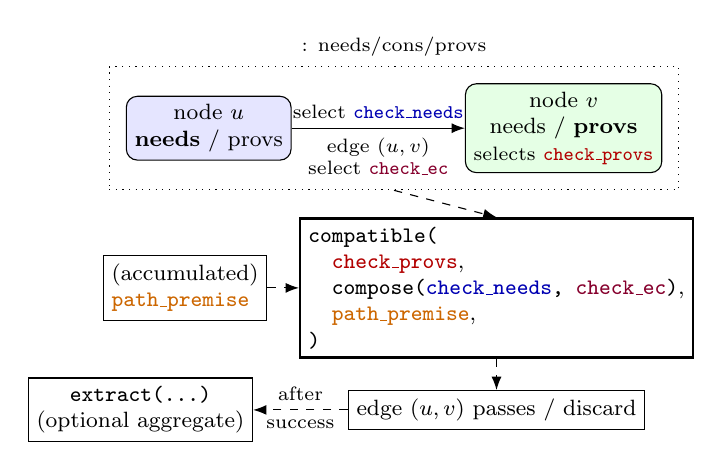
\begin{tikzpicture}[
  font=\footnotesize,
  node distance=8mm,
  u/.style={draw, rounded corners, fill=blue!10, align=center, inner sep=3pt},
  v/.style={draw, rounded corners, fill=green!10, align=center, inner sep=3pt},
  boxext/.style={draw, rectangle, align=left, inner sep=3pt},
  lbl/.style={font=\scriptsize},
  ->, >=Latex
]
\node[u] (u) {node $u$ \\ \textbf{needs} / provs};
\node[v, right=22mm of u] (v) {node $v$ \\ needs / \textbf{provs}\\{\scriptsize selects \textcolor{red!70!black}{\texttt{check\_provs}}}};
\node[draw, dotted, rectangle, fit=(u)(v), inner sep=6pt,
      label=above:{\scriptsize \sysgraph: needs/cons/provs}] (sel) {};
% path premise
\node[boxext] (path) [below=12mm of u, xshift=-3mm] {(accumulated) \\ \textcolor{orange!80!black}{$\texttt{path\_premise}$}};
% compat
\node[boxext, align=left, thick] (compat) [right=4mm of path] {%
\texttt{compatible(}\\
\quad \textcolor{red!70!black}{\texttt{check\_provs}},\\
\quad \texttt{compose(}\textcolor{blue!70!black}{\texttt{check\_needs}}\texttt{, }\textcolor{purple!70!black}{\texttt{check\_ec}}\texttt{)},\\
\quad \textcolor{orange!80!black}{\texttt{path\_premise}},\\
\texttt{)}};
% result
\node[boxext, align=center] (ok) [below=4mm of compat] {edge $(u,v)$ passes / discard};
% extract
\node[boxext, align=center] (extract) [left=12mm of ok] {\texttt{extract(...)}\\(optional aggregate)};
% inside app graph
\draw[->]
  (u) -- node[lbl, above] {select \textcolor{blue!70!black}{\texttt{check\_needs}}}
        node[lbl, below, align=center] {edge $(u,v)$\\select \textcolor{purple!70!black}{\texttt{check\_ec}}} (v);
% app graph to compatible args
\draw[->, dashed] (sel.south) -- (compat.north);
% path premise into compatible
\draw[->, dashed] (path.east) -- node[lbl, above] {} (compat.west);
% result
\draw[->, dashed] (compat) -- (ok);
\draw[->, dashed] (ok.west) -- node[lbl, above] {after} node[lbl, below] {success} (extract.east);

\end{tikzpicture}
%\vspace{-0.1in}
        \caption{Example flow for a single edge $(u,v)$: inside \sysgraph, select \texttt{check\_needs}, \texttt{check\_ec}, and the node’s \texttt{check\_provs}; outside, evaluate \texttt{compatible} on \texttt{compose(check\_needs, check\_ec)} and \texttt{path\_premise}. After a successful compatibility check, \texttt{extract} function can optionally aggregate \texttt{compatible} return value. For multigraphs, repeat per parallel edge (or edge combinations) with its own \texttt{cons} tuple. Solid arrows are part of \sysgraph and have the same meaning as the figures below. Dashed arrows represent control flow.}
\label{fig:skel}
\end{wrapfigure}


In the implementation (also see Fig. \ref{fig:skel}), we perform a depth-first search (DFS) starting from a
given source node, keeping track of visited edges and the accumulated
constraints in \texttt{path\_premise}, along the current path.
Constraints in \texttt{path\_premise} are invisible to users and are dynamic in nature based on which
edge(s), \texttt{needs}, \texttt{provs} are selected. Constraints are populated in and out
based on the satisfiability of the previous levels, and current level checks.
\sysname{} perform compatibility checks, \texttt{compatible(check\_provs,
compose(check\_needs, check\_ec), path\_premise)}:
for each edge $(u, v)$ from the current node $u$, it checks if \texttt{provs} from $v$
and \texttt{cons} from edge $(u, v)$ satisfy needs from $u$.
This checks if the chosen path satisfies the guarantees required by the destination
(\texttt{check\_provs}) is
implied by the conjunction (the result returned from call to \texttt{compose}) of the chosen needs of the
source (\texttt{check\_needs}) and the chosen edge constraints
(\texttt{check\_ec}),
considering the constraints already accumulated (\texttt{path\_premise}).
If all checks succeed, the application is deemed compatible
with the plugged-in \sysmods{} and the application logics are also
sound as a whole.


To avoid redundant checks in case of a subset of nodes and edges needs to be reused for scalability,
\sysname{} can aggretate a subgraph into a single logical node using the \texttt{extract} function.
% \jiyong{Does this previous sentence make sense?}
% \jiyong{What is composability check? Is it compatibility check or compositional check or something else?}
% same thing, prob missed it when revising the terms
After a successful compositional check, \texttt{extract} processes the resulting graph
representing a valid assignment of constraints, and outputs a single summary node.
This node encapsulates the net semantic guarantee of the subgraph reachable from the 
\texttt{entry} node, provided there are no external edges crossing the subgraph boundary.
The function performs a DFS starting from \texttt{entry} to compute this summary.
For each edge (\texttt{src}, \texttt{dst})
traversed in the DFS, the extraction function uses the specific \texttt{provs}
constraint assigned to \texttt{src} in the result graph, uses the specific
needs constraint assigned to \texttt{dst} in the provided graph, and retrieves
\texttt{cons} constraint assigned to the edge in
the argument graph. The extract function creates a composite constraint
for this single edge interaction: \texttt{compose(src\_provs, edge\_cons,
dst\_needs)}. This represents the conjunction of constraints relevant
to this specific step in the flow. It collects these composite
constraints from all edges reachable from subgraph root in the DFS. Finally,
it returns the logical \textsc{and} of all collected composite
constraints. Simply put, axioms and relations define constraints on
operations; similarly, \texttt{extract} defines a summary constraint on a
successfully composed subgraph. If the compositional check found a valid
way for components A, B, and C to interact starting from A,
\texttt{extract(A, graph)}---the first argument is aggregated subgraph's root node and the second is the return result from 
\texttt{compose} call, containing the full graph's nodes and edges---%
%(first argument is aggregate node's constraint flow entrance, second is the exit.
%Current implementation requires the first two arguments to be identical.
%The third is the return result from \texttt{compose} call, containing the full graph's nodes and edges)
% \jiyong{What does each arguement represent and how do they connect to components A B and C?}
generates a single formula representing the
overall guarantee provided by the A $\,\to\,$ B $\,\to\,$ C chain, as seen from A's
perspective, based on the specific choices made during the compositional check.
% Previously checked results are reusable with the above introduced extraction function
% \jiyong{If we do DFS do we ever get to reuse the checked results?}
%  not here because the "reuse" i mean is that, once the new aggregate node is created
% users can re-create a new full appgraph, so the intermediate steps of are skipped
% in new checks
By replacing a verified subgraph with its summary node, \sysname{} enables modular verification.
Subsequent checks on the full application graph can treat this summary as a primitive component,
thereby bypassing the internal complexity of the original subgraph and improving solver scalability.

\subsection{Compatible Combination Search}
\label{subsec:search}

\sysname{} is capable of searching for compatible \sysmods{} for an
application given an \sysgraph{}. When blank \sysmods{} are plugged into the
\sysgraph{}, \sysname{} searches for compatible combinations of
\sysmods{} for the user.
Considering that strictly weaker distributed semantics can be replaced
with strictly stronger ones and the weaker semantics are typically
more performant and cheaper to maintain, \sysname{} searches the space
in an order that prioritizes weaker semantics. Specifically, we give scores
0 to 5 to semantics in the columns from left to right in
\cref{fig:semantics-tree}
and test the combination that has lower sum of scores first during the search.
If compatible combinations are found, the search can stop early; replacing a
\sysmod{} in a compatible combination with a strictly stronger one is always
guaranteed to be compatible.
However, our search strategy is not optimal and investigating more
efficient search algorithms remains as future work.

%If a compatible combination is found that satisfies all unvisited edges
%between u and v at the current step, it adds the chosen constraints
%(needs, provs, cons) to the result graph, updates the path\_premise
%by composing the newly satisfied constraints, marks the edges as
%visited, and continues the DFS from the destination node v. If the
%DFS eventually visits all edges in the graph, the function returns
%True and the result graph showing one valid assignment. If a dead end
%is reached or no compatible combination works for an edge, it
%backtracks, removing the choices made at that step and trying other
%combinations. If the DFS completes without visiting all edges
%(meaning no fully consistent assignment was found), it returns False.
